\documentclass[10pt, aspectratio=1610, natbib, handout]{beamer}
\usepackage{common}

\title[Web Scraping]{
  \textbf{Web Scraping and Data Tools}
}

\subtitle[Macro 3: TA\#6]{
  \textbf{Macroeconomics 3:} TA class \#6
}

\author[A.~Pasqualini]{
  Andrea Pasqualini
}

\institute[Bocconi]{Bocconi University}

\date{
  15 March 2021
}

\begin{document}

  \begin{frame}
    \maketitle
  \end{frame}

  \begin{frame}
    \frametitle{Web Scraping: What Is It?}

    \begin{block}{Definition}
      From Wikipedia:
      \textit{
        Web Scraping [...] is used for extracting data from websites. [...]
        The term typically refers to automated processes implemented using a bot or web crawler.
        It is a form of copying in which specific data is gathered and copied from the web, typically into a central local database or spreadsheet, for later retrieval or analysis.
      }
    \end{block}

    \vfill\pause

    \textbf{Objective:}
    Build a dataset from potentially unstructured data stored on a remote (web) server

    \textbf{Tools:}
    Computer programs that navigate, identify and organize data into a structured dataset

  \end{frame}

  \begin{frame}
    \frametitle{Web Scraping: Why?}

    \begin{itemize}
      \item Limited availability of structured data
        \begin{itemize}
          \item Structured data are records assembled by somebody (e.g., gov't agency)
          \item Cost of assembling records is high (e.g., data entry, data verification, methodologies)
          \item Benefit must outweigh the costs
        \end{itemize}

      \vfill\pause

      \item The Internet as a medium of information exchange
        \begin{itemize}
          \item The Internet grew fast because it's a business opportunity (e.g., Amazon)
          \item Information is available for consumption reasons
          \item Assembling structured \textit{public} datasets carries little value for stakeholders
        \end{itemize}

      \vfill\pause

      \item The Internet as a platform for user-generated content
        \begin{itemize}
          \item Users generate massive amounts of coded information (e.g., eBay)
          \item Users generate massive amounts of uncoded information (e.g., Twitter)
        \end{itemize}
    \end{itemize}

    \vfill\pause

    \textbf{Catch-all reason:} uncover new evidence with novel data

    \textbf{Relevant reading:} \cite{Edelman2012}

  \end{frame}

  \begin{frame}
    \frametitle{Web Scraping: Examples (from Edelman, 2012)}

    \textbf{Microeconomics}
    \begin{itemize}
      \item \textbf{Patrick Bajari and Ali Hortacsu.} 2003. ``The Winner's Curse, Reserve Prices, and Endogenous Entry: Empirical Insights from eBay Auctions.'' \textit{RAND Journal of Economics} 34(2): 329--55.
      \item Bid data from coin sales on eBay reveal bidder behavior in auctions, including the magnitude of the winner's curse
    \end{itemize}

    \vfill\pause

    \textbf{Macroeconomics}
    \begin{itemize}
      \item \textbf{Alberto Cavallo.} 2015. ``Scraped Data and Sticky Prices.'' \textit{NBER Working Paper}
      \item Daily price data from online supermarkets reveal price adjustment and price stickiness
    \end{itemize}

    \vfill\pause

    \textbf{Financial Economics}
    \begin{itemize}
      \item \textbf{Werner Antweiler and Murray Z.~Frank.} 2004. ``Is All That Talk Just Noise? The Information Content of Internet Stock Message Boards.'' \textit{Journal of Finance} 59(3): 1259--94.
      \item Finds that online discussions help predict market volatility; effects on stock returns are statistically significant but economically small
    \end{itemize}

    % \vfill\pause

    % \textbf{Labor and Demographic Economics}
    % \begin{itemize}
    %   \item \textbf{Benjamin Edelman.} 2012. ``Earnings and Ratings at Google Answers.'' \textit{Economic Inquiry} 50(2): 309--320
    %   \item Measures labor market outcomes in an online research service, including higher earnings for experience, flexibility, and disfavored work schedules
    % \end{itemize}

    % \vfill\pause

    % \textbf{Industrial Organization}
    % \begin{itemize}
    %   \item \textbf{Judith Chevalier and Austan Goolsbee.} 2003. ``Measuring Prices and Price Competition Online: Amazon.com vs.~BarnesandNoble.com.'' \textit{Quantitative Marketing and Economics} 1(2): 203--222
    %   \item Uses publicly available price and rank data to estimate demand elasticities at two leading sellers of online books, finding greater price sensitivity at Barnes \& Noble than at Amazon
    % \end{itemize}

  \end{frame}

  \begin{frame}
    \frametitle{Web Scraping: Which Tools and When to Use Them?}


    % \textbf{Copy-paste}
    %   \begin{itemize}
    %     \item Basic human interaction, not automated, rarely fails, zero learning curve
    %   \end{itemize}

    % \vfill\pause

    % \textbf{Text pattern matching}
    %   \begin{itemize}
    %     \item Grab a text, use programs to find/wrangle keywords (e.g., \texttt{grep}, \texttt{awk}, \texttt{sed})
    %   \end{itemize}

    % \vfill\pause

    \textbf{HTTP programming}  \hfill\dimmer{(HTTP: HyperText Transfer Protocol)}
      \begin{itemize}
        \item Carefully craft a willful URL
        \item Obtain and manage response from server
        \item Most popular: HTTP Application Programming Interfaces (API)
      \end{itemize}

    \vfill\pause

    \textbf{HTML parsing}  \hfill\dimmer{(HTML: HyperText Markup Language)}
      \begin{itemize}
        \item Write a program to ``surf'' specific HTML code
        \item Navigate to specific points
        \item Read and write info on separate data storage
      \end{itemize}

    \vfill\pause

    \textbf{Browser automation}  \hfill\dimmer{(DOM: Document Object Model)}
      \begin{itemize}
        \item Write a program to hijack your browser
        \item Make the browser navigate webpages, read and write info
        \item Useful for dynamically-generated HTML pages (e.g., Twitter)
      \end{itemize}

  \end{frame}

  \begin{frame}
    \frametitle{The Internet: A Primer at Light Speed (1/3)}

    What happens when you write a URL in the address bar and press Enter?

    \begin{enumerate}
      \item Your browser sends a \textbf{HTTP request} for data to the destination web server
      \item The web server receives the request and\dots\ serves it, sending a \textbf{HTTP response} back
      \item Your browser receives the data, analyzes the metadata, and displays a payload
    \end{enumerate}

    \vfill\pause

    A \textbf{HTTP request} is a text file with the following components
    \begin{itemize}
      \item A request line
      \item Request header fields
      \item An empty line
      \item (Optional) A message body
    \end{itemize}

    \vfill\pause

    A \textbf{HTTP response} is a text file with the following components
    \begin{itemize}
      \item A status line
      \item Response header fields
      \item An empty line
      \item (Optional) A message body
    \end{itemize}

  \end{frame}

  \begin{frame}[fragile]
    \frametitle{The Internet: A Primer at Light Speed (2/3)}

    \begin{columns}
      \begin{column}{0.35\textwidth}
        \textbf{Example HTTP request}
      \end{column}
      \begin{column}{0.60\textwidth}
        \begin{lstlisting}[language=HTML]
          GET / HTTP/1.1
          Host: www.example.com

        \end{lstlisting}
      \end{column}
    \end{columns}

    \vfill\pause

    \begin{columns}
      \begin{column}{0.35\textwidth}
        \textbf{Example HTTP response} \\
        \# 1      --- Status line   \\
        \# 2--9   --- Header fields \\
        \# 11--18 --- Message body

        \vspace{1em}

        \begin{table}
          \centering
          \begin{tabular}{cl}
            \toprule
            Status       & Meaning      \\
            \midrule
            \texttt{1xx} & Information  \\
            \texttt{2xx} & Success      \\
            \texttt{3xx} & Redirection  \\
            \texttt{4xx} & Client error \\
            \texttt{5xx} & Server error \\
            \bottomrule
          \end{tabular}
        \end{table}
      \end{column}
      \begin{column}{0.60\textwidth}
        \begin{lstlisting}[language=HTML]
          HTTP/1.1 200 OK
          Date: Mon, 23 May 2005 22:38:34 GMT
          Content-Type: text/html; charset=UTF-8
          Content-Length: 155
          Last-Modified: Wed, 08 Jan 2003 23:11:55 GMT
          Server: Apache/1.3.3.7 (Unix) (Red-Hat/Linux)
          ETag: "3f80f-1b6-3e1cb03b"
          Accept-Ranges: bytes
          Connection: close

          <html>
            <head>
              <title>An Example Page</title>
            </head>
            <body>
              <p>Hello World, this is a HTML document.</p>
            </body>
          </html>
        \end{lstlisting}
      \end{column}
    \end{columns}

  \end{frame}

  \begin{frame}
    \frametitle{The Internet: A Primer at Light Speed (3/3)}

    Why do we care about HTTP requests and responses?

    \vfill\pause

    \textbf{HTTP programming}
    \begin{itemize}
      \item The response message body is the data we are after (e.g., API)
      \item Can be a \{ JSON, CSV, XLS, \dots\ \} file
    \end{itemize}

    \vfill\pause

    \textbf{HTML parsing}
    \begin{itemize}
      \item The response message body is (static) HTML code
      \item We use a program to parse the HTML code
    \end{itemize}

    \vfill\pause

    \textbf{Browser automation}
    \begin{itemize}
      \item The response message body may contain a \texttt{<script>} tag (e.g., JavaScript)
      \item The HTML code changes dynamically depending on circumstances
      \item Cannot handle this with a simple HTML parser
    \end{itemize}

    \vfill\pause

    Luckily, Python can handle each and every of these scenarios!

  \end{frame}

  \begin{frame}
    \frametitle{Web Scraping: The Tools in the Python Toolbox}

    \textbf{HTTP programming}
    \begin{itemize}
      \item \alert{\texttt{import requests}}
      \item Craft custom requests
      \item Manage responses
      \item \url{https://requests.readthedocs.io/en/master/}
    \end{itemize}

    \vfill\pause

    \textbf{HTML parsing}
    \begin{itemize}
      \item \alert{\texttt{import bs4}}
      \item Access the HTML code in a response's message body
      \item Navigate the HTML document with a ``Pythonic'' interface
      \item \url{https://www.crummy.com/software/BeautifulSoup/bs4/doc/}
    \end{itemize}

    \vfill\pause

    \textbf{Browser automation}
    \begin{itemize}
      \item \alert{\texttt{import selenium}}
      \item Hijack your web browser, emulate human behavior with a browser
      \item Navigate the potentially-changing HTML document, trigger functions in web scripts
      \item \url{https://selenium-python.readthedocs.io/}
    \end{itemize}

  \end{frame}

  \begin{frame}[fragile]
    \frametitle{HTTP Programming: An Example}

    Go to \url{https://xkcd.com/2434/info.0.json} (write a HTTP request)

    \vfill\pause

    The message body of the HTTP response is (this is the pretty-print)

    \begin{lstlisting}
      {
        "month": "3",
        "num": 2434,
        "link": "",
        "year": "2021",
        "news": "",
        "safe_title": "Vaccine Guidance",
        "transcript": "",
        "alt": "I can't wait until I'm fully vaccinated and can safely send chat messages in all caps again.",
        "img": "https://imgs.xkcd.com/comics/vaccine_guidance.png",
        "title": "Vaccine Guidance",
        "day": "8"
      }
    \end{lstlisting}

    \vfill\pause

    All we need to do is
    \begin{itemize}
      \item Translate this JSON text into a Python dictionary
      \item Feed the dictionary into a \texttt{pandas.DataFrame}
    \end{itemize}

    \vfill

    \dimmer{I have permission to do this: see \texttt{https://xkcd.com/license.html}.}

  \end{frame}

  \begin{frame}
    \frametitle{HTML Parsing / Browser Automation: Identifying Information}

    All website content is embedded into its HTML document

    \vfill\pause

    \textbf{Objective:} identify information of interest in the HTML tree

    \vfill\pause

    \begin{itemize}
      \item Use \textit{Web Developer Tools} in your browser to easily identify elements in the HTML tree
      \item Take notes: what HTML tags are used? How are elements \textit{uniquely} identified?
    \end{itemize}

    \vfill\pause

    My experience
    \begin{itemize}
      \item Tidy websites uniquely identify elements with CSS classes
      \item Messy websites require smart strategies (e.g., find table whose caption is [smth])
      \item Some web developers intentionally make seemingly messy HTML code
        \begin{itemize}
          \item Web dev laziness, and/or
          \item Sophisticated back-end design (e.g., Facebook), and/or
          \item Deliberate attempt at making scraping difficult
        \end{itemize}
    \end{itemize}

  \end{frame}

  \begin{frame}
    \frametitle{HTML Parsing / Browser Automation: Example (1/2)}

    \begin{figure}
      \centering
      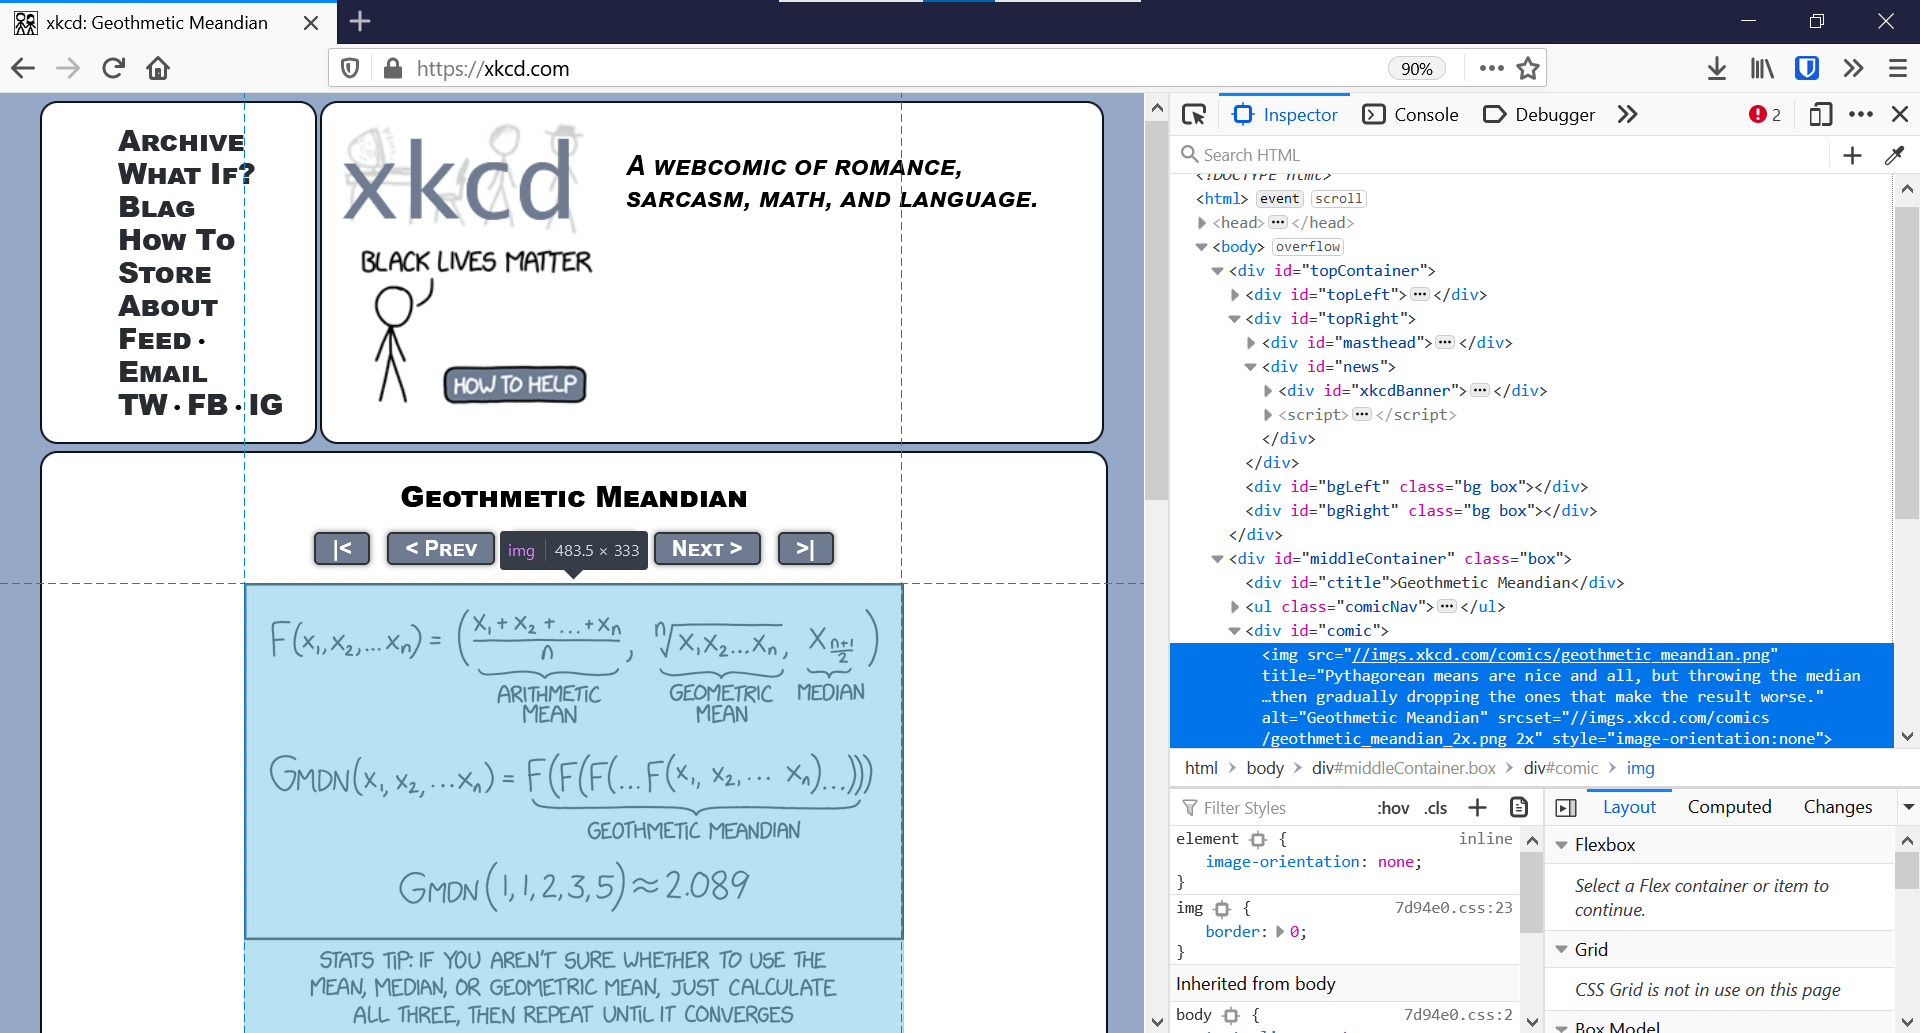
\includegraphics[width=\textwidth]{./assets/xkcd-home.png}
    \end{figure}

    \vfill

    \dimmer{I have permission to do this: see \texttt{https://xkcd.com/license.html}.}

  \end{frame}

  \begin{frame}
    \frametitle{HTML Parsing / Browser Automation: Example (2/2)}

    \begin{figure}
      \centering
      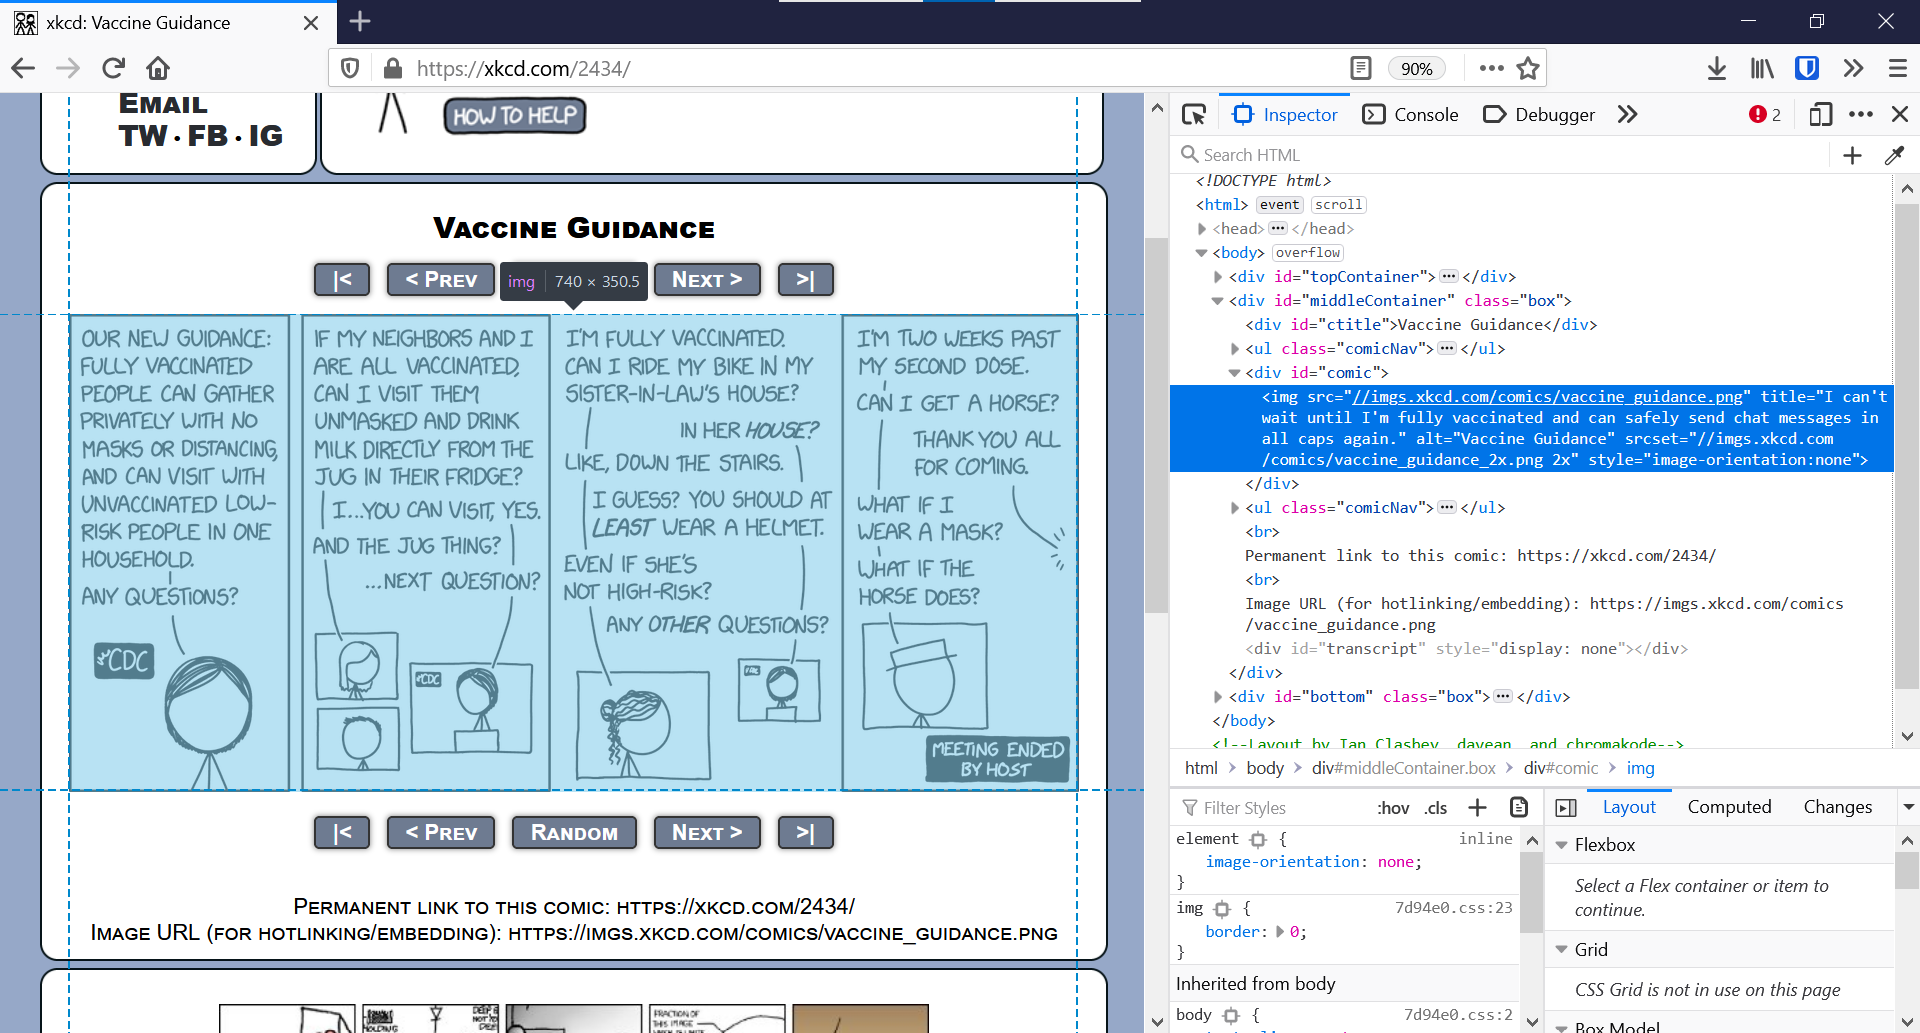
\includegraphics[width=\textwidth]{./assets/xkcd-2434.png}
    \end{figure}

    \vfill

    \dimmer{I have permission to do this: see \texttt{https://xkcd.com/license.html}.}

  \end{frame}

  \begin{frame}
    \frametitle{Web Scraping: Beware!}

    \begin{center}
      \textbf{THIS SLIDE DOES NOT CONSTITUTE LEGAL ADVICE.}
    \end{center}

    \vfill\pause

    \begin{itemize}
      \item Web scraping may be illegal in your jurisdiction
      \item Web scraping may be forbidden by a website's Terms and Conditions
      \item Web scraping may be used to collect sensitive personal information
    \end{itemize}

    \vfill\pause

    It is important to take adequate precautions
    \begin{itemize}
      \item Read the Terms and Conditions
      \item Ask for permission to the website owner (see, ``webmaster'')
      \item Seek advice from your University / Institution / Human Studies committee
    \end{itemize}

  \end{frame}

  \begin{frame}
    \frametitle{Web Scraped! \dots\ Now What?}

    \begin{itemize}
      \item Keep the code for scraping separate from the rest
      \vfill\pause
      \item Store the resulting (raw) dataset on disk, label it with a date
      \vfill\pause
      \item Clean the dataset (will take a lot of time)
      \vfill\pause
      \item Keep the code for cleaning separate from the rest
      \vfill\pause
      \item Store the resulting (clean) dataset on disk
      \vfill\pause
      \item Research away!
    \end{itemize}

  \end{frame}

  \begin{frame}
    \frametitle{Practice Time}

    Moving to a Jupyter Notebook

  \end{frame}

  \begin{frame}
    \frametitle{Wrapping up my TA Classes: What to Remember for the Exam}

    \begin{itemize}
      \item Solving Bellman Equation for the fixed point $V(\cdot)$
        \begin{itemize}
          \item Value Function Iter., Policy Function Iter.~(i.e., Howard's Improvement), Direct Projection
          \item Mind the \textit{Curse of Dimensionality}
          \item Policy functions are generally well-behaved (e.g., capital accumulation almost linear)
        \end{itemize}
      \vfill\pause
      \item Adding exogenous stochastic variables
        \begin{itemize}
          \item Tauchen, Tauchen-Hussey, Rouwenhorst are limited to AR(1) processes
          \item Literature has come up with approaches for general continuous Markov processes
        \end{itemize}
      \vfill\pause
      \item Solving for the equilibrium prices
        \begin{itemize}
          \item Define the net excess demand
          \item Take it to zero with a zero-finding routine
        \end{itemize}
      \vfill\pause
      \item Solving for equilibrium prices with heterogeneous agents
        \begin{itemize}
          \item Combine exogenous transition matrix with policy functions
          \item Obtain endogenous transition matrix across the whole vector of state variables
          \item Compute the ergodic distribution
          \item Aggregate agents and define aggregate demand minus aggregate supply
        \end{itemize}
      \vfill\pause
      \item Combining idiosyncratic and aggregate shocks
        \begin{itemize}
          \item Computationally expensive, but feasible (esp.~by mixing projection and perturbation methods)
          \item Consider MIT shocks: IRF to ``parameters'' using only idiosyncratic uncertainty
        \end{itemize}
    \end{itemize}

  \end{frame}

  \begin{frame}
    \frametitle{Wrapping up my TA Classes: What to Remember for the Profession}

    I hope I gave you

    \vfill\pause

    \begin{itemize}
      \item A glimpse into numerical methods in Economics
      \vfill\pause
      \item A clear understanding of our reliance on computing, as Economists
      \vfill\pause
      \item A solid foundation into projection methods and models with heterogeneous agents
      \vfill\pause
      \item A sense of curiosity for ``robustness'' exercises
      \vfill\pause
      \item An idea of how much Python can be flexible and powerful
    \end{itemize}

    \vfill\pause

    Tip: when you work with code, do like this guy: \url{https://github.com/michaelstepner/healthinequality-code/blob/master/code/readme.md}

  \end{frame}

  \appendix

  \begin{frame}
    \frametitle{References}

    \bibliographystyle{apalike}
    \bibliography{references}

  \end{frame}


\end{document}
